\problemname{The Kangaroo Mother}

\begin{figure}[!h]
\begin{center}
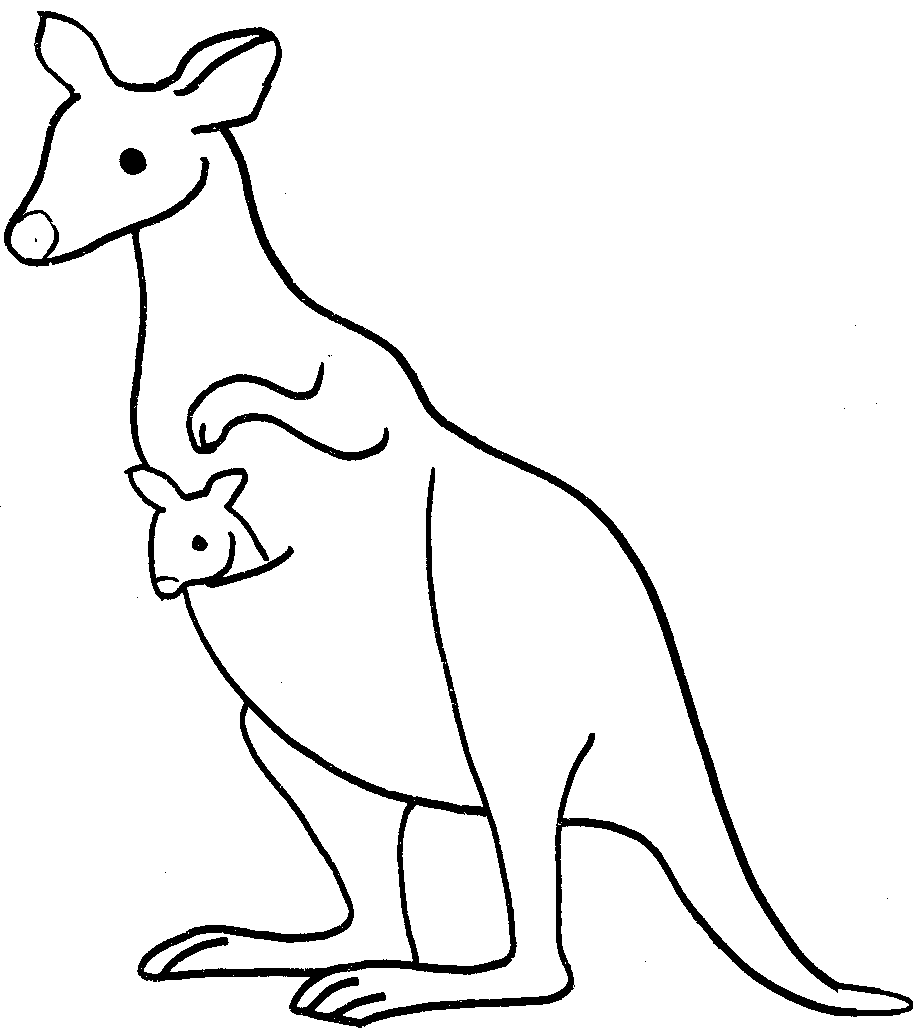
\includegraphics[width=0.3\textwidth]{kangaroo.png} 
\end{center}
\end{figure}

A kangaroo mother is packing her children into her pouch. She has lots of
children. The two smallest weigh only one gram each, but then each child
weighs as much as the two previous ones combined. Her six smallest children
thus weigh 1, 1, 2, 3, 5, and 8 grams.

The mother can carry at most $X$ kilograms (and not even one gram more). How many children can she bring?

\section*{Input}

The input consists of a line with an integer $X$, where $1\le X \le 1000$, the
maximum number of kilograms the mother can carry.

\section*{Output}

The program should output a line with an integer, the maximum number of children
that together weigh at most $X$ kilograms.
